% !TeX program = tectonic
\documentclass[utf8, a4paper, 12pt]{ctexart}

\usepackage{fontspec}
\usepackage[margin=1in]{geometry}
\usepackage{graphicx}
\usepackage{amsmath}
\usepackage{amssymb}
\usepackage{booktabs}
\usepackage{longtable}
\usepackage{array}
\usepackage{tabularx}
\usepackage{float}
\usepackage{caption}
\usepackage{subcaption}
\usepackage{hyperref}
\usepackage{xurl}
\usepackage{setspace}
\usepackage{makecell}
\usepackage{enumitem}
\usepackage{tikz}
\usetikzlibrary{arrows.meta,calc,positioning}

\hypersetup{
    colorlinks=true,
    linkcolor=black,
    citecolor=black,
    urlcolor=blue
}

\setlength{\parindent}{2em}
\setlength{\parskip}{0.3em}
\setstretch{1.25}
\setlength{\emergencystretch}{2em}
\renewcommand{\arraystretch}{1.15}
\renewcommand{\UrlFont}{\ttfamily\small}
\graphicspath{{Figures/}}

\ctexset{
    section = {
        format = \Large\bfseries\raggedright,
    },
    subsection = {
        format = \large\bfseries\raggedright
    }
}

\newcolumntype{L}[1]{>{\raggedright\arraybackslash}p{#1}}
\newcolumntype{C}[1]{>{\centering\arraybackslash}p{#1}}
\newcolumntype{Y}{>{\raggedright\arraybackslash}X}

\tikzset{
    seq participant/.style={
        draw,
        rounded corners=2pt,
        fill=black!5,
        minimum width=1.75cm,
        minimum height=0.72cm,
        align=center,
        font=\scriptsize
    },
    seq lifeline/.style={gray!60, dashed},
    seq call/.style={-{Latex[length=2mm,width=1.2mm]}, semithick},
    seq reply/.style={-{Latex[length=2mm,width=1.2mm]}, semithick, dashed},
    seq note/.style={
        draw,
        rounded corners=2pt,
        fill=yellow!12,
        text width=3.9cm,
        align=left,
        inner sep=3pt,
        font=\scriptsize
    },
    seq note wide/.style={
        draw,
        rounded corners=2pt,
        fill=yellow!12,
        text width=6.8cm,
        align=left,
        inner sep=3pt,
        font=\scriptsize
    }
}

\newcommand{\onlineSequenceFigure}{
\begin{tikzpicture}[x=1cm,y=1cm]
    \node[seq participant] (bag) at (0.0,0) {rosbag};
    \node[seq participant] (fl) at (2.3,0) {FAST-LIO};
    \node[seq participant] (br) at (4.6,0) {pose\\bridge};
    \node[seq participant] (pp) at (6.9,0) {PointPillars};
    \node[seq participant] (mc) at (9.2,0) {MCTrack};
    \node[seq participant] (jb) at (11.5,0) {joint\\backend\\ego};
    \node[seq participant] (out) at (13.8,0) {RViz /\\Recorder};

    \foreach \p in {bag,fl,br,pp,mc,jb,out} {
        \draw[seq lifeline] (\p.south) -- ++(0,-15.8);
    }

    \draw[seq call]
        ($(bag.south)+(0,-0.9)$) --
        node[above,font=\scriptsize] {发布 IMU + 原始 LiDAR(t)}
        ($(fl.south)+(0,-0.9)$);

    \node[seq note, anchor=west] at (2.85,-1.55) {preprocess() 首先冻结前一个\\\texttt{tracked\_objects} 快照，并降低\\动态盒内点的权重。};

    \draw[seq call]
        ($(fl.south)+(0,-2.6)$) to[out=15,in=345,looseness=7]
        node[right,font=\scriptsize,align=left] {IMU 传播、扫描去畸变、\\地图匹配以及 EKF 更新}
        ($(fl.south)+(0,-3.2)$);

    \node[seq note, anchor=west] at (2.85,-4.0) {同时发布 \texttt{/Odometry\_imu\_predicted}\\作为 LiDAR 更新前的预测位姿接口。};

    \draw[seq reply]
        ($(fl.south)+(0,-4.85)$) --
        node[above,font=\scriptsize] {\texttt{/Odometry}(t)}
        ($(br.south)+(0,-4.85)$);

    \draw[seq reply]
        ($(br.south)+(0,-5.7)$) --
        node[above,font=\scriptsize] {\texttt{/mctrack/lidar\_pose}(t)}
        ($(mc.south)+(0,-5.7)$);

    \draw[seq call]
        ($(bag.south)+(0,-6.6)$) --
        node[above,font=\scriptsize] {同步发布 LiDAR(t)}
        ($(pp.south)+(0,-6.6)$);

    \draw[seq reply]
        ($(pp.south)+(0,-7.45)$) --
        node[above,font=\scriptsize] {\texttt{/detection/lidar\_detections}(t)}
        ($(mc.south)+(0,-7.45)$);

    \draw[seq call]
        ($(mc.south)+(0,-8.35)$) to[out=15,in=345,looseness=7]
        node[right,font=\scriptsize,align=left] {根据检测时间戳查询 \texttt{pose\_buffer}；\\必要时进行插值或短暂等待}
        ($(mc.south)+(0,-8.95)$);

    \draw[seq call]
        ($(mc.south)+(0,-9.75)$) to[out=15,in=345,looseness=7]
        node[right,font=\scriptsize,align=left] {更新跟踪器并输出世界系/雷达系\\下的对象状态}
        ($(mc.south)+(0,-10.35)$);

    \draw[seq reply]
        ($(mc.south)+(0,-11.15)$) --
        node[above,font=\scriptsize] {\texttt{/mctrack/tracked\_objects}(t)}
        ($(fl.south)+(0,-11.15)$);

    \draw[seq reply]
        ($(mc.south)+(0,-12.0)$) --
        node[above,font=\scriptsize] {\texttt{/mctrack/tracked\_objects}(t)}
        ($(jb.south)+(0,-12.0)$);

    \draw[seq reply]
        ($(fl.south)+(0,-12.85)$) --
        node[above,font=\scriptsize] {\texttt{/Odometry}(t)}
        ($(jb.south)+(0,-12.85)$);

    \draw[seq call]
        ($(jb.south)+(0,-13.7)$) to[out=15,in=345,looseness=7]
        node[right,font=\scriptsize,align=left] {当前自位姿的滑窗优化}
        ($(jb.south)+(0,-14.3)$);

    \draw[seq reply]
        ($(jb.south)+(0,-15.1)$) --
        node[above,font=\scriptsize] {\texttt{/joint\_backend/odom}(t)}
        ($(out.south)+(0,-15.1)$);

    \node[seq note wide, anchor=west] at (4.1,-15.95) {\texttt{tracked\_objects}(t) 不会追溯性修改当前扫描 $t$；\\相反，它成为下一帧 FAST-LIO 动态降权链的输入。};
\end{tikzpicture}
}

\newcommand{\onlineResultFigure}[1]{
\begin{figure}[!h]
    \centering
    \begin{subfigure}[t]{0.49\textwidth}
        \centering
        
\includegraphics[width=\linewidth]{../Results/#1_results/Online/evaluation_result.png}
        \caption{在线前端对比}
    \end{subfigure}
    \hfill
    \begin{subfigure}[t]{0.49\textwidth}
        \centering
        
\includegraphics[width=\linewidth]{../Results/#1_results/Online/evaluation_joint_backend.png}
        \caption{联合后端评估}
    \end{subfigure}

    \vspace{0.8em}

    \begin{subfigure}[t]{0.58\textwidth}
        \centering
        
\includegraphics[width=\linewidth]{../Results/#1_results/Online/ablation_bar.png}
        \caption{ATE/RPE 柱状对比}
    \end{subfigure}
    \caption{序列 #1 的完整在线实验结果。}
\end{figure}
}

\title{基于多目标跟踪（MOT）的自动驾驶激光 SLAM 系统}
\author{ME5400 项目组}
\date{\today}

\makeatletter
\newcommand{\makecoverpage}{
\begin{titlepage}
    \centering
    \vspace*{2.0cm}
    
\includegraphics[width=0.58\textwidth]{nus_logo_cover.jpg}\par

    \vspace{2.6cm}
    {\bfseries\fontsize{22}{30}\selectfont
    \parbox{0.9\textwidth}{\centering \@title}\par}

    \vfill
    {\Large \@author \par}
    \vspace{0.8cm}
    {\large \@date \par}
\end{titlepage}
}
\makeatother

\begin{document}
\hypersetup{pageanchor=false}
\makecoverpage
\hypersetup{pageanchor=true}
\tableofcontents
\newpage
\setcounter{page}{1}

\begin{abstract}
本报告详尽阐述了 ME5400 课程项目——面向动态场景下的激光 SLAM 与多目标跟踪（MOT）系统。该系统集成了用于激光惯性自运动估计的 FAST-LIO、用于 3D 目标检测的 PointPillars 以及用于在线轨迹关联和运动状态估计的 MCTrack。其核心思想是构建一个双向闭环而非单向串联：FAST-LIO 提供的位姿稳定了 MCTrack 的关联，而跟踪到的目标状态被转化为 FAST-LIO 中的软动态权重，并作为对象一致性因子引入仅包含自车位姿（ego-only）的滑窗后端中。

所有定量讨论均基于 \texttt{Results/} 目录下 7 个 KITTI 跟踪序列（0003, 0006, 0007, 0009, 0010, 0013, 0020）的归档在线实验结果。报告强调算法设计意图与工程实现细节，包括 ROS 接口、时间同步、位姿缓冲、标准结果归档以及失效模式分析。在所有 7 个序列中，前端配置 \texttt{FAST-LIO+MCTrack} 在 ATE RMSE 指标上均始终优于纯 FAST-LIO 基线，表明最可靠的增益源自“位姿辅助跟踪”与“跟踪反馈式动态降权”形成的前端闭环。联合后端虽在部分漂移严重的序列上有所帮助，但其稳定性较弱，在速度外推、时间戳对齐或目标门控不可靠时可能失效，序列 0009 便是最典型的例子。本报告的总体结论采用了审慎的态度：本项目并非追求 SOTA 的联合 SLAMMOT 系统，而是一个可复现的工程原型，它验证了定位-跟踪反馈闭环的可行性，并为未来向以对象为中心（object-centric）的联合优化转型奠定了基础。
\end{abstract}

\noindent\textbf{关键词：} FAST-LIO；PointPillars；MCTrack；动态场景 SLAM；多目标跟踪；面向对象的感知；ROS 重现性

\section{引言与背景}
在动态道路场景中进行定位与感知，往往面临着一对此消彼长且难以调和的矛盾。激光 SLAM 及激光惯性里程计的基础假设是所观测到的大部分几何特征是静态、可重复见且可长期复用的。其前端扫描匹配、局部地图维护及后端一致性保障，均高度依赖于“当前时刻观测到的点所对应的表面在后续帧中依然具有几何意义”这一前提。然而，自动驾驶感知系统最关注的对象（如周边车辆、行人、骑行者等）却恰恰违背了这一假设。换言之，在语义层层面对决策至关重要的区域，在几何层面往往对传统的 SLAM 系统构成了巨大威胁。这一冲突催生了大量关于动态场景 SLAM 的研究，从早期的通过检测并过滤运动区域的视觉系统，到近期能够联合推理自运动与目标轨迹的 SLAMMOT 管线~\cite{staticfusion,ds-slam,dynaslam,limot,dl-slot}。

动态目标对激光 SLAM 的负面影响并非仅仅是“运动点是离群值”那么简单，而是通过至少三个耦合的退化通道起作用。首先是\textbf{地图污染（map contamination）}：运动车辆的点被当作静态表面插入局部或全局地图中，导致系统积累“鬼影”结构、双重墙体或拖尾，误导后续帧的配准。其次是\textbf{配准退化（registration degradation）}：即使这些点尚未永久融合进地图，如果当前帧配准残差中有很大比例由运动物体产生，局部优化器就会被迫去拟合不一致的几何结构，从而使当前帧的位姿估计产生偏差。最后是\textbf{漂移累积（drift accumulation）}：随着时间推移，上述两个问题会互相放大——微小的帧间修正偏差会扭曲局部地图，进而导致后续修正效果进一步恶化，最终产生持久的轨迹偏移。因此，动态场景不仅仅是增加了随机噪声，而是改变了优化问题本身的结构。

现有的动态场景 SLAM 系统通常采用以下三种策略之一。第一类尝试通过语义分割、运动一致性测试或鲁棒损失函数完全剔除动态点。当动态目标占视野比例较小时，该策略往往非常有效，但在大型车辆占主导的拥挤交通场景中，这可能会丢弃过多有用的几何结构。第二类尝试更显式地分离静态层与动态层，例如在稠密 RGB-D 管线中采用加权背景融合，或在视觉 SLAM 中进行语义前景过滤~\cite{staticfusion,ds-slam,dynaslam}。第三类也是更新的一类，将目标状态视为一等变量，追求自运动与被跟踪目标之间的某种程度的联合优化~\cite{confslammot,limot,imm-slammot,online-dynamic-slam,dl-slot}。对于本项目而言，实际的问题在于一个学期规模的工程系统应该如何切入这一设计空间。

多目标跟踪（MOT）面临着与之相反但同样重要的依赖关系。跟踪器通常被描述为对“检测”进行操作，但仅靠 3D 检测不足以跨帧提供稳定的运动估计。当自车本身在移动时，每一个检测结果都必须经过自车运动补偿（ego-motion compensation）才能被正确解读；否则，一个在世界系下静止的目标会看起来在移动，而一个平稳移动的目标则可能出现跳变。这不仅影响关联，还影响融合速度、加速度及跟踪置信度等衍生指标。如果位姿流存在噪声，跟踪器在世界系下的运动估计也会随之不准。反之，如果跟踪器无法维持连贯的 ID 和速度轨迹，它也无法为定位堆栈提供可靠的反馈。因此，两者之间的关系本质上是双向的：更好的定位能改善跟踪，而更好的跟踪可以通过识别哪些点应被赋予较低权重，或通过提供额外的目标级约束来改善定位。

本项目正是植根于这一双向直觉。系统采用 FAST-LIO~\cite{fastlio2} 作为激光惯性定位主干，PointPillars~\cite{pointpillars} 作为 3D 检测器，MCTrack 作为在线跟踪器以生成目标 ID、融合速度、加速度及轨迹长度。FAST-LIO 发布优化里程计与 IMU 预测运动。桥接节点将这些输出转换为 MCTrack 所需的位姿格式。PointPillars 按时间戳发布 3D 检测消息。MCTrack 消费检测与位姿，执行经运动补偿的关联，并发布跟踪目标。这些跟踪目标随后通过两种方式被利用：一是转化为软动态权重，在下一帧 FAST-LIO 扫描中降低动态包围盒内点的权重；二是送入仅含自车位姿（ego-only）的联合后端，测试稳定的目标观测能否为自车轨迹提供额外的滑窗约束。这一设计虽然尚未构成统一的因子图，但已形成了一个完整的信息闭环。

在工程实践中，我们有两项设计选择需要简要说明。首先是采用\textbf{软降权（soft down-weighting）}而非硬剔除，因为硬删除在误报、框抖动、遮挡或暂时静止的情况下显得过于脆弱。其次是选择从一个\textbf{松耦合的工程闭环}起步，而非紧耦合的对象中心图。完整的联合图在理论上更优雅，但其所需的因子设计、置信度建模、边缘化处理及调试工作量远超本课程项目的周期。

据此，本项目追求四个关联的目标。\textbf{研究目标}是测试定位与跟踪在不构建完整统一优化器的情况下，能否在动态驾驶场景中形成有意义的反馈闭环。\textbf{工程目标}是构建一个可运行的 ROS 管线，其组件、消息契约、启动顺序、结果日志及评估脚本均是显式且可复现的。\textbf{评估目标}是确定闭环中哪一部分提供了最稳定的收益：是前端权重环节、后端修正环节，还是两者兼有。\textbf{诊断目标}是识别阻碍当前系统表现得像一个鲁棒的联合 SLAMMOT 方案的具体失效模式。

具体而言，本报告及实现的贡献可总结如下：
\begin{itemize}[leftmargin=2em]
    \item 实现了 FAST-LIO、PointPillars、MCTrack 与 ego-only 后端的完整 ROS 集成，采用项目定义的标准消息接口而非临时私有接口。
    \item 构建了前端闭环：FAST-LIO 位姿稳定了 MCTrack，而 MCTrack 的输出在 FAST-LIO 预处理中转化为点级软权重。
    \item 建立了可复现的实验框架，支持基线与优化运行的一键切换、\texttt{Results/} 下的标准归档、TUM 格式轨迹记录及统一的定量评估。
    \item 通过失效感知分析表明，前端闭环是最稳定的改进源，而当前的后端在速度外推及时间不确定性面前仍显脆弱。
\end{itemize}

选择 KITTI Tracking 作为主要验证数据集是深思熟虑的结果。KITTI 为真实的城市驾驶场景提供了同步的激光雷达、IMU、标定信息及自车运动真值~\cite{kitti}。其 Tracking 切片包含测试定位-跟踪闭环所需的动态车辆、轨迹变化及背景演变。本文使用的 7 个在线序列（0003, 0006, 0007, 0009, 0010, 0013, 0020）涵盖了不同的漂移水平、动态强度及相对轨迹跨度。本报告并非追求全数据集的榜单排名，而是分析该系统在那些日志、图表及轨迹文件均可直接复现和检查的序列上的表现。

这一立场引出了一个重要的定位说明：\textbf{本报告并非旨在声称达到了 SOTA 性能}。它记录的是一个验证了双向定位-跟踪闭环可行性、展示了完整实验管线并使失效案例透明化的工程原型。对于课程项目而言，这种集成质量、可重复性及诊断能力本身就是极具价值的成果。一个端到端运行、可多序列回放并能准确暴露失效原因的系统，比一个未经充分调试、仅在表面上显得“紧耦合”的方案更能为后续研究打下坚实基础。

\section{研究现状分析}
为了更准确地定位本项目，必须从两个维度讨论相关工作。第一类是\textbf{动态场景 SLAM}，其重点在于检测、过滤或联合建模运动区域，以保持定位与建图的稳定性。第二类是\textbf{面向自动驾驶的 3D MOT}，其重点在于在自车运动下维持准确的目标轨迹和运动状态。本项目处于这两者的交汇点：它既不是单纯的动态物体过滤系统，也不是一个完整的以对象为中心的联合优化器。因此，一个有意义的对比需要考虑传感器配置、前端形式、耦合程度、动态物体处理策略、实时性倾向以及工程复杂度。

\begin{table}[H]
    \centering
    \caption{与本项目相关的代表性动态场景 SLAM 及 3D MOT 工作对比}
    \label{tab:slammot_related_work}
    \small
    \begin{tabularx}{\textwidth}{p{1.9cm} p{2.5cm} p{2.2cm} p{2.5cm} X}
        \toprule
        工作 & 传感器 / 前端 & 耦合方式 & 动态处理 / 实时性 & 与本项目的关联 \\
        \midrule
        StaticFusion & RGB-D; 稠密直接法 SLAM & 联合估计相机运动与分割 & 加权背景融合; 实时稠密建图~\cite{staticfusion} & 展示了采用软降权及保留背景结构而非单纯硬剔除的价值。 \\
        DS-SLAM & 视觉; ORB-SLAM2 + 语义线程 & 松耦合多线程设计 & 语义过滤加运动一致性; 面向实时运行~\cite{ds-slam} & 证明了模块化、多线程的工程结构仍能提高动态场景下的鲁棒性。 \\
        DynaSLAM & 视觉; ORB-SLAM2 家族 & 侧重过滤, 恢复静态图 & 动态检测加背景修复; 较慢但精确~\cite{dynaslam} & 阐明了将动态目标主要视为待移除区域s的优势与局限。 \\
        Conf SLAMMOT & 激光; 激光里程计 & 紧耦合因子图 & 优化内部的置信度引导关联~\cite{confslammot} & 启发了后续基于置信度的对象因子权重设计。 \\
        LIMOT & 激光+惯性; 自研 LIO & 紧耦合滑窗因子图 & 实时联合激光惯性里程计与 MOT~\cite{limot} & 是本项目在超越话题级耦合后，最接近的高层目标架构。 \\
        IMM-SLAMMOT & 双目视觉; ORB-SLAM2 & 紧耦合 BA & 显式的目标运动模型切换~\cite{imm-slammot} & 强调了在交通场景中，单一的恒定速度模型往往是不够的。 \\
        Online Dynamic SLAM & 双目视觉; 自研 VO & 紧耦合增量平滑 & 基于 iSAM2 的在线动态优化~\cite{online-dynamic-slam} & 指出了为什么增量式后端对于可扩展性和稳定性至关重要。 \\
        DL-SLOT & 激光; 激光里程计 & 紧耦合协同图优化 & 定位与跟踪之间的滑窗协同~\cite{dl-slot} & 为激光侧的窗口管理和对象因子集成提供了相关参考。 \\
        AB3DMOT & 激光检测; 简单 KF 跟踪器 & 无 SLAM 耦合 & 3D 卡尔曼滤波加匈牙利匹配; 极速~\cite{ab3dmot} & 代表了许多实际 MOT 管线背后的轻量级跟踪哲学。 \\
        CenterPoint & 激光; 基于中心的检测/跟踪 & 检测-跟踪集成, 无 SLAM 耦合 & 利用中心速度实现简单且强大的跟踪~\cite{centerpoint} & 在讨论 MCTrack 的检测器-跟踪器设计选择时作为重要的对比基线。 \\
        \bottomrule
    \end{tabularx}
\end{table}

\subsection{从动态点剔除到动态感知估计}
StaticFusion、DS-SLAM 和 DynaSLAM 共同定义了动态场景 SLAM 的早期演进~\cite{staticfusion,ds-slam,dynaslam}。尽管它们使用的是 RGB-D 或视觉前端而非激光惯性估计，但它们确立了三个至今依然适用的理念：应显式检测动态区域；应保守地保留背景结构而非盲目删除；模块化系统在不将所有内容合并为单一优化器的情况下仍能改善鲁棒性。相对于本项目，它们的共同局限在于动态物体主要被视为需要抑制或避开的区域，而非具备运动属性、后续可能帮助定位的跟踪实体。当前系统与之不同的是，在过滤之后依然保持了对象级信息的存续。

\subsection{近期 SLAMMOT 系统与向联合优化的推进}
Conf SLAMMOT、LIMOT、IMM-SLAMMOT、Online Dynamic SLAM 和 DL-SLOT 集体展示了该领域当前的发展方向~\cite{confslammot,limot,imm-slammot,online-dynamic-slam,dl-slot}。这些工作不再将 SLAM 和 MOT 视为孤立的黑盒。相反，它们共享状态、关联置信度、运动先验或优化窗口。最重要的共同趋势是从“先定位、后跟踪”的流水线转向一种对象状态、置信度与自运动在同一估计过程中互相补全的联合系统。

Conf SLAMMOT 特别值得关注，因为它强调了优化过程内部的置信度引导关联~\cite{confslammot}。这对本项目很有意义，因为目前的后端仍使用相对简单的权重（主要基于检测得分 and 轨迹长度）。Conf SLAMMOT 传达的底层信息是：置信度不应仅仅是保留或丢弃对象的阈值，它应该影响对应因子的强度。这正是本项目后端如果要提高在不稳定序列上的鲁棒性所需演进的方向。

LIMOT 可能是本项目预想的长期目标最接近的参考~\cite{limot}。它在一个紧耦合的滑动窗口框架内集成了激光惯性里程计与多目标跟踪，是当前基于话题设计的直接对照。与 LIMOT 相比，本项目目前的统一性明显不足：FAST-LIO、PointPillars、MCTrack 和后端仍然通过消息交换而非共享单一状态图。然而，这种对比并非纯粹负面的。由于本项目已经在模块边界发布了必要的信息（包括带时间戳的位姿、雷达系对象观测、世界系跟踪状态、得分与运动属性），它实际上已经组装了紧耦合公式所需的大部分数据。

IMM-SLAMMOT 通过强调动态目标的多种运动模型贡献了不同的经验~\cite{imm-slammot}。交通参与者并不都遵循单一整齐的匀速模式。汽车会停止、加速和转弯；行人的行为更难以预测。本项目继承了 MCTrack 在线模式下的实用匀速行为，这对于第一个工程原型是足够的，但一旦这些跟踪速度被用作后端约束，就会暴露出局限。在某些序列（尤其是 Sequence 0009）中观察到的性能下降，一定程度上可以通过这一视角来理解：后端信任了基于过于简单模型生成的运动外推。

Online Dynamic SLAM 值得注意，因为它专注于动态场景中的增量平滑与建图，而非仅仅是批处理式的滑动窗口~\cite{online-dynamic-slam}。其对本项目的启发不在于具体的传感器模态（它是视觉而非激光惯性），而在架构设计经验上：一旦动态信息进入估计问题，窗口管理、增量更新和计算可扩展性就会成为设计的核心。目前 ME5400 的后端仍使用通过非线性最小二乘重复求解的 ego-only 小窗口。这是一个合理的中间阶段设计，但尚未触及真实在线联合 SLAMMOT 系统必须解决的长效扩展问题。

DL-SLOT 在激光雷达侧极具启发性，因为它探索了动态激光 SLAM 与 3D 目标跟踪之间的协同图优化~\cite{dl-slot}。相对于本项目，DL-SLOT 代表了相同通用目标的更成熟版本：它不在外部接口层对话，而是在优化层共享信息。这使得 DL-SLOT 成为后续后端演进的有用指南，特别是关于对象相关约束应如何在窗口中调度、加权和边缘化。

\subsection{纯 3D MOT 背景与跟踪主干的选择}
MOT 文献之所以重要，是因为对象信息的可用性取决于这些信息是如何产生的。AB3DMOT 和 CenterPoint 代表了两种实用的设计哲学~\cite{ab3dmot,centerpoint}：一种强调在检测之上进行轻量级的卡尔曼式跟踪，另一种则将更多运动信息推入射向器-跟踪器内部。对于本项目而言，关键的对比不在于哪种基准测试最强，而在于哪种接口对下游最有用。MCTrack 的吸引力在于它暴露了轨迹长度、融合速度、速度变化、加速度及稳定 ID，所有这些都能直接复用于动态降权及后端门控。

\subsection{对比分析与存在的差距}
从这些工作中可以归纳出三个宏观观察。首先，\textbf{该领域正朝着更紧密的耦合方向发展}：最强大的近期系统不再保持 SLAM 和 MOT 的完全分离。其次，\textbf{动态物体处理仍主要集中在过滤、关联 and 对象状态估计}；即使是联合系统也并不总是能将动态物体作为自车定位的几何支撑。第三，\textbf{实时性与工程复杂度依然是决定性因素}，因为随着耦合程度增加，同步、置信度建模与稳定优化变得更加困难。

相对于上述研究格局，本项目占据了一个有意为之的中间位置。它已经实现了一个真实的双向反馈闭环，因此超越了单向级联管线；但它仍然是一个侧重工程的松耦合原型，而非完整的以对象为中心的联合优化器。其价值在于解决了许多方案中隐晦提及的接口与复现性问题：带时间戳的消息、同步、坐标变换、实验编排、标准化日志以及多序列失效分析。存在的差距是明确的：系统已经具备了未来联合优化器所需的\textbf{信息流}，但尚未具备充分利用这些流的\textbf{状态表示}与\textbf{因子设计}。

\section{整体系统架构、PointPillars / MCTrack 与数据流}
\begin{figure}[H]
    \centering
    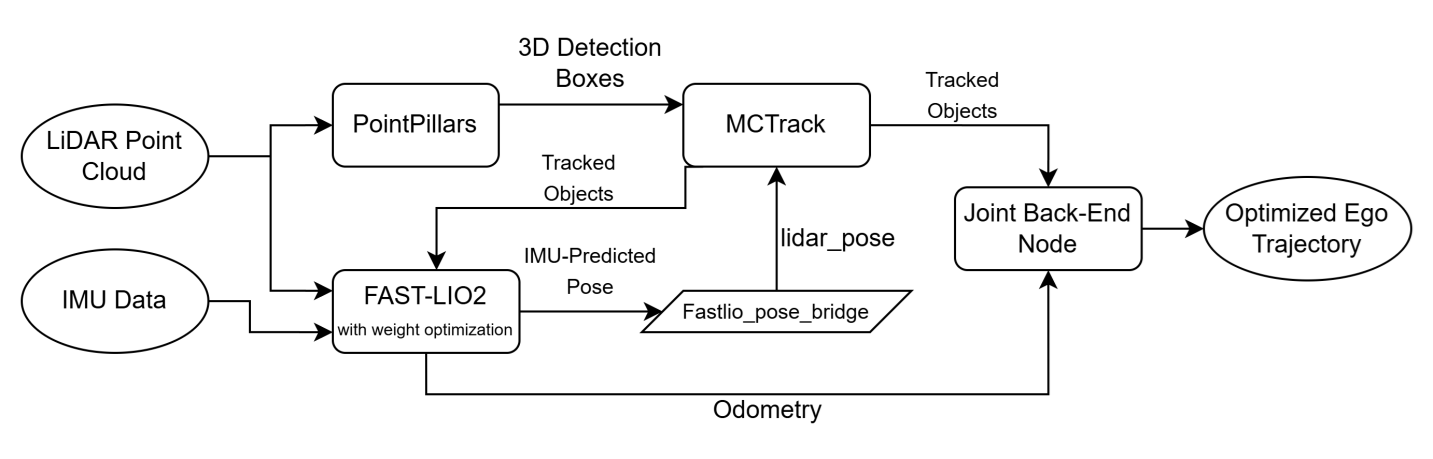
\includegraphics[width=0.96\textwidth]{Overall architecture of the proposed dynamic-scene trajectory optimization framework.png}
    \caption{整体系统架构。可以将其解读为感知先行、跟踪对齐紧随其后、联合修正最后的三个层次的过程。}
    \label{fig:overall_architecture}
\end{figure}

图~\ref{fig:overall_architecture} 作为一个数据依赖图比作为静态方框图更容易理解。第一层执行感知与自运动估计：FAST-LIO 发布位姿，而 PointPillars 从相同的激光雷达输入发布 3D 检测。第二层执行时空对齐：\texttt{fastlio\_pose\_bridge.py} 将 FAST-LIO 里程计转换为 MCTrack 所需的激光位姿接口，MCTrack 将位姿与检测对齐以形成连贯的目标轨迹。第三层执行反馈与修正：跟踪到的目标被送回 FAST-LIO 开启动态点降权，并送往自车后端进行窗口化轨迹修正。

这种组织形式是必要的，因为各模块运行在不同层级上。FAST-LIO 处理原始几何与惯性传播，PointPillars 处理学习到的目标假设，MCTrack 处理时间关联，后端处理短时域的自车修正。保持这些阶段显式化有助于避免阻塞行为，并使增益或失效能够更容易地追溯到具体接口。

如果从数据流视角理解系统，过程可总结为以下七步：
\begin{enumerate}[leftmargin=2.2em]
    \item 传感器首先获取原始激光点云与 IMU 数据，并同时输入 FAST-LIO 和 PointPillars。
    \item PointPillars 产生当前帧的 3D 检测，指出附近存在哪些目标。
    \item FAST-LIO 输出当前自位位姿，并持续提供高频运动预测。
    \item 位姿桥接节点将这些定位输出转换为跟踪模块直接可用的格式。
    \item MCTrack 结合“观测到了什么”与“自车如何运动”来完成目标关联、轨迹更新及速度估计。
    \item 跟踪输出反馈给 FAST-LIO，以便对可能属于动态目标的点进行降权。
    \item 同样的跟踪输出也被送入联合后端，以进一步精修自车轨迹。
\end{enumerate}

这一七步描述已经说明了为什么系统必须组织为一个有向但延迟的闭环。轨迹在检测关联之前无法存在，动态点权重在跟踪消息存在之前也无法计算。因此，时刻 \(t\) 产生的跟踪状态影响的是后续扫描而非当前扫描。这一帧的延迟并非缺陷，而是保证闭环能够在线运行且不产生循环阻塞的关键。

\subsection{FAST-LIO 前端}
\begin{figure}[H]
    \centering
    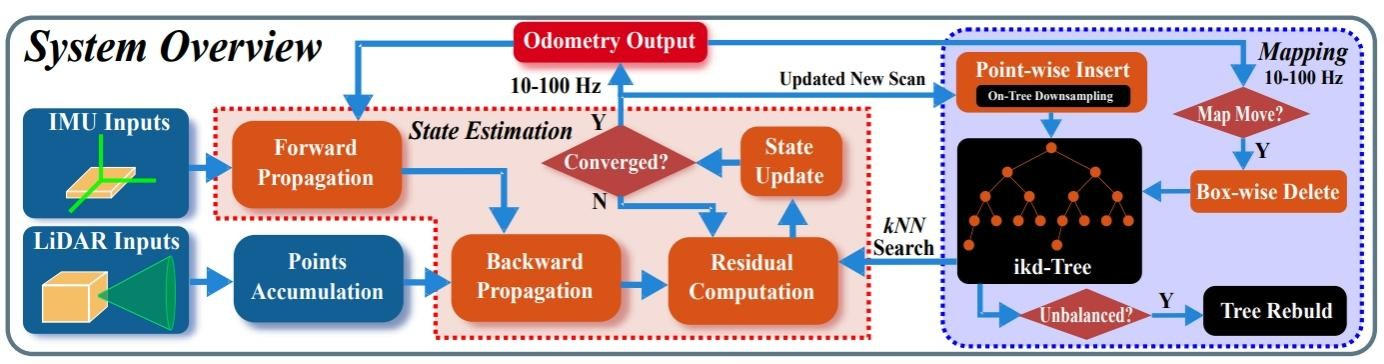
\includegraphics[width=0.82\textwidth]{FAST-LIO2 System Architecture.jpg}
    \caption{FAST-LIO2 前端架构。本项目中，来自 MCTrack 的对象信息被注入点云预处理管线，实现对动态点的自适应降权。}
    \label{fig:fastlio_architecture}
\end{figure}

FAST-LIO 是整个系统的定位主干，也是上述数据流中的起点。它直接消费来自 KITTI rosbag 的激光点云与 IMU 数据，内部使用紧耦合的激光惯性估计管线输出稳定的自车位姿。本项目中，FAST-LIO 不仅产生全局一致的 \texttt{/Odometry}，还发布 \texttt{/Odometry\_imu\_predicted} 作为高频预测位姿，为后续跟踪与后端优化提供统一参考。

从模块职责看，FAST-LIO 在系统中扮演三个角色。首先，它为 MCTrack 提供可靠的自车位姿，使得 3D 检测在跨帧关联前能完成自运动补偿。其次，它为联合后端提供原始里程计约束，使后端优化不至于偏离前端估计过远。第三，通过 \texttt{preprocess.cpp} 及 \texttt{laserMapping.cpp} 中的跟踪对象回调路径，它接收 \texttt{/mctrack/tracked\_objects}，将其转换为内部 \texttt{DynamicObject} 结构，并将目标运动属性映射为点级权重。因此，FAST-LIO 既是自运动信息的源头，也是对象反馈最直接地改变扫描级几何处理的地方。

从算法角度看，FAST-LIO 前端可以理解为一个结合了 IMU 传播与激光几何修正的迭代滤波器。设系统状态为 \(\mathbf{x}_k\)，IMU 输入为 \(\mathbf{u}_k\)。预测步可写为：
\begin{equation}
\mathbf{x}_{k+1|k}=f(\mathbf{x}_{k|k}, \mathbf{u}_k)+\mathbf{w}_k,
\qquad
\mathbf{P}_{k+1|k}=\mathbf{F}_k \mathbf{P}_{k|k}\mathbf{F}_k^\top+\mathbf{Q}_k,
\end{equation}
其中 \(\mathbf{P}\) 为状态协方差，\(\mathbf{F}_k\) 为线性化状态转移矩阵。对于当前帧中的第 \(j\) 个点，FAST-LIO 进一步利用局部地图中的参考平面构建点到面的几何残差：
\begin{equation}
r_j=\mathbf{n}_j^\top\!\bigl(\mathbf{R}(\mathbf{x})\,\mathbf{p}_j+\mathbf{t}(\mathbf{x})-\mathbf{q}_j\bigr),
\end{equation}
并通过迭代更新来最小化：
\begin{equation}
\delta \mathbf{x}^{\star}
=
\arg\min_{\delta \mathbf{x}}
\left(
\sum_{j} \|r_j\|^2_{\mathbf{\Sigma}_j^{-1}}
+\;
\|\delta \mathbf{x}\|^2_{\mathbf{P}_{k+1|k}^{-1}}
\right).
\end{equation}
这些公式描述了 FAST-LIO 在本项目中的核心作用：IMU 提供高频连续预测，激光点云残差将位姿拉回几何一致的解。这就是为什么 FAST-LIO 既能稳定输出 \texttt{/Odometry}，又能充当 MCTrack 的时空参考。

为了将 FAST-LIO 的输出接入跟踪模块，项目实现了 \texttt{fastlio\_pose\_bridge.py}，它利用配置的机体系到雷达系外参将 \texttt{/Odometry} 转换为 \texttt{/mctrack/lidar\_pose} 并以 TF 形式发布。这一显式桥接使得定位、跟踪与可视化保持一致的坐标系约定。FAST-LIO 在预处理每一帧扫描前会将最新的跟踪对象冻结为扫描局部快照，因此每个点都是针对一致的对象集合进行加权的，而不是针对中途变动的消息缓冲区。

\subsection{PointPillars 检测模块}
PointPillars~\cite{pointpillars} 通过 \texttt{MMDET3D/local/ros/nodes/kitti\_pointpillars\_bag\_node.py} 包装为 ROS 节点，能够直接消费来自 rosbag 的 KITTI 点云。其角色不仅仅是输出原始检测，而是为整个系统提供统一、可溯源且带时间戳的 3D 检测消息。项目在 \texttt{catkin\_ws/src/ME5400/msg/Detection3D.msg} 和 \texttt{Detection3DArray.msg} 中定义了统一消息格式，包含帧 ID、类别、置信度、2D 框、3D 尺寸、雷达系位置及偏航角。这样，PointPillars 与 MCTrack 不依赖任何私有第三方格式，而是通过项目定义的消息接口进行通信。

\begin{figure}[H]
    \centering
    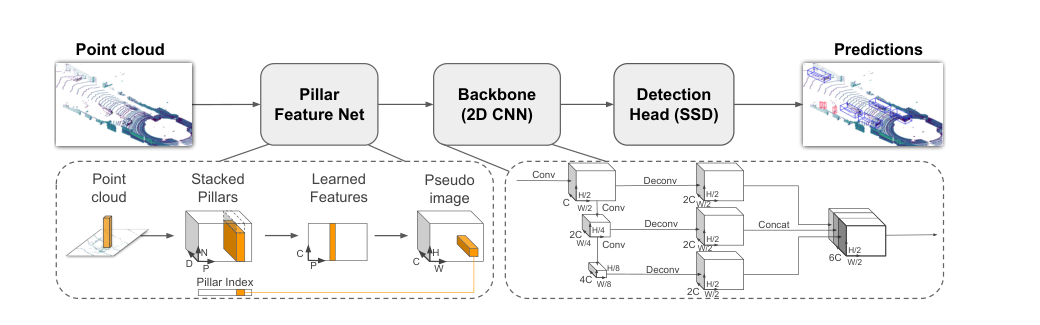
\includegraphics[width=0.95\textwidth]{PointPillars Network Architecture.png}
    \caption{来自原始 PointPillars 论文的网络架构。该网络由 Pillar Feature Net、2D CNN 主干和 SSD 检测头组成。图像转载自 Lang \textit{et al.} 的 CVPR 2019 论文~\cite{pointpillars}。}
    \label{fig:pointpillars_architecture}
\end{figure}

PointPillars 的本质是通过编码垂直柱（pillars）将稀疏 3D 点云转换为 BEV 伪图像，然后应用 2D CNN 检测头。这把昂贵的 3D 卷积问题转化为了廉价的 2D 卷积，这也是为什么 PointPillars 能够满足当前在线系统的实时性要求。

用公式表示，若第 \(l\) 个 pillar 包含点集 \(\mathcal{P}_l=\{\mathbf{p}_i\}\)，PointPillars 首先为每个点构造增强特征：
\begin{equation}
\tilde{\mathbf{p}}_i=
\bigl[
x_i,\; y_i,\; z_i,\; r_i,\;
x_i-\bar{x}_l,\; y_i-\bar{y}_l,\; z_i-\bar{z}_l,\;
x_i-x_l^c,\; y_i-y_l^c
\bigr],
\end{equation}
其中 \((\bar{x}_l,\bar{y}_l,\bar{z}_l)\) 是 pillar 内点的均值，\((x_l^c,y_l^c)\) 是 pillar 中心。经过 Pillar Feature Net 后，pillar 级特征可写为：
\begin{equation}
\mathbf{f}_l=\max_{i\in \mathcal{P}_l}\phi(\tilde{\mathbf{p}}_i),
\end{equation}
随后将其散射到 BEV 伪图像中：
\begin{equation}
\mathbf{I}(u,v)=
\begin{cases}
\mathbf{f}_l, & (u,v)=\mathrm{index}(l),\\
\mathbf{0}, & \text{否则},
\end{cases}
\end{equation}
最后，检测头联合优化分类、框回归与朝向预测：
\begin{equation}
\mathcal{L}_{\mathrm{det}}
=
\beta_{\mathrm{cls}}\mathcal{L}_{\mathrm{cls}}
+\beta_{\mathrm{loc}}\mathcal{L}_{\mathrm{loc}}
+\beta_{\mathrm{dir}}\mathcal{L}_{\mathrm{dir}}.
\end{equation}

从工程视角看，这一设计服务于三个目的：保持标定一致性；维持较低检测门限以便后续通过跟踪与门控进行裁剪；暴露可被 MCTrack、可视化及评估重用的统一消息契约。PointPillars 有意不解决内部跟踪，其工作是发布具有时间戳和得分的几何 3D 假设，以便后续失效可被更清晰地回溯。

\subsection{MCTrack 模块与数据流细节}
\begin{figure}[H]
    \centering
    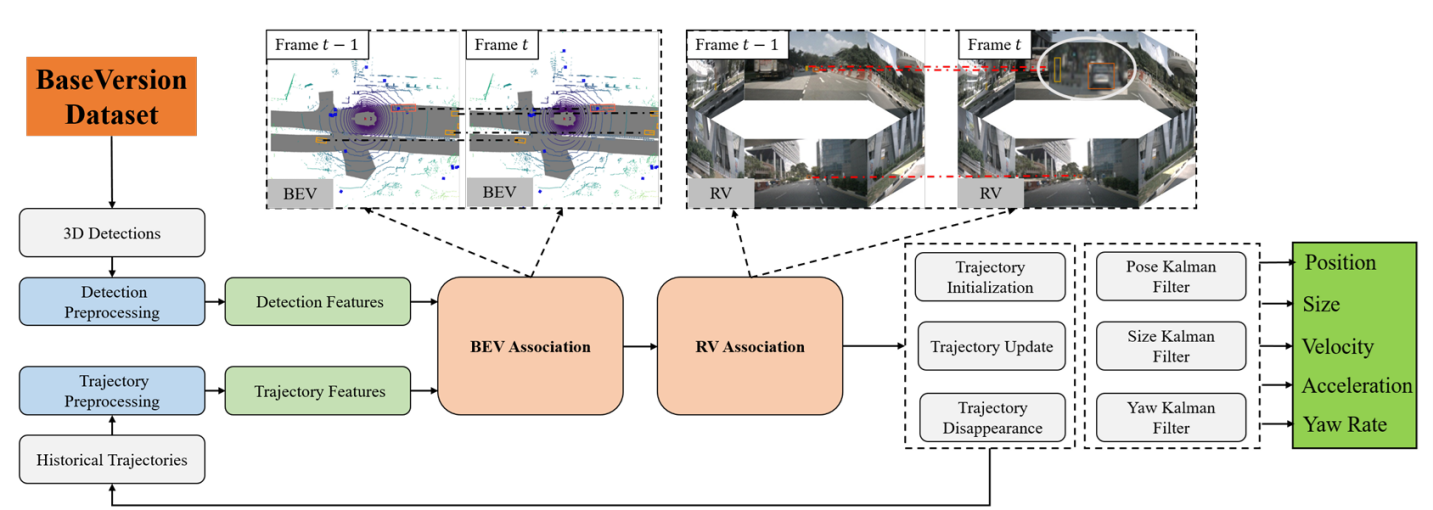
\includegraphics[width=0.92\textwidth]{Overview of 3D MOT framework MCTrack.png}
    \caption{MCTrack 3D MOT 框架示意图。其输出不仅包含位置和尺寸，还包含速度、加速度、轨迹长度及相关运动属性。}
    \label{fig:mctrack_framework}
\end{figure}

在线 MCTrack 节点实现在 \texttt{catkin\_ws/src/ME5400/scripts/mctrack\_online\_node.py} 中。它默认订阅 \texttt{/mctrack/lidar\_pose} 和 \texttt{/detection/lidar\_detections}，内部维护位姿缓冲区和待处理检测队列，仅在合适时间戳的位姿可用后才处理检测。这种“检测等待位姿、位姿驱动处理”的设计避免了纯按到达顺序处理导致的跨帧关联的时间错位。

MCTrack 同时发布可视化用的 \texttt{/mctrack/markers} 和下游优化用的 \texttt{/mctrack/tracked\_objects}。在 \texttt{TrackedObject.msg} 中，除了对象位姿和尺寸，还记录了 \texttt{track\_length}、\texttt{velocity}、\texttt{velocity\_fusion}、\texttt{velocity\_diff}、\texttt{velocity\_curve} 和 \texttt{acceleration}。这些字段非常关键，因为随后的动态权重优化和联合后端门控均依赖运动属性而非仅仅框位置。

在当前的 \texttt{kitti\_fastlio.yaml} 配置下，MCTrack 在线模式的主状态估计可近似为 2D 匀速卡尔曼滤波。若轨迹状态为：
\begin{equation}
\mathbf{x}_k=[p_x,\; p_y,\; v_x,\; v_y]^\top,
\end{equation}
其预测模型为：
\begin{equation}
\mathbf{x}_{k|k-1}=
\begin{bmatrix}
1 & 0 & \Delta t & 0\\
0 & 1 & 0 & \Delta t\\
0 & 0 & 1 & 0\\
0 & 0 & 0 & 1
\end{bmatrix}
\mathbf{x}_{k-1|k-1},
\qquad
\mathbf{H}=
\begin{bmatrix}
1 & 0 & 0 & 0\\
0 & 1 & 0 & 0
\end{bmatrix},
\qquad
\mathbf{z}_k=\mathbf{H}\mathbf{x}_{k|k-1}+\mathbf{v}_k,
\end{equation}
随后执行标准卡尔曼更新。在数据关联层，当前在线配置主要采用基于预测框的 3D 代价矩阵及匈牙利匹配：
\begin{equation}
\mathcal{A}^{\star}
=
\arg\min_{\mathcal{A}\in\Pi}
\sum_{(i,j)\in\mathcal{A}} C_{ij},
\qquad
C_{ij}=1-\mathrm{RO\mbox{-}GDIOU}_{3D}\!\left(\hat{B}_i,\; B_j\right),
\end{equation}
其中 \(\hat{B}_i\) 为轨迹预测框，\(B_j\) 为当前检测框。换言之，FAST-LIO 首先通过自运动位姿稳定了跨帧几何，随后 MCTrack 通过运动预测与全局最优匹配将离散检测转换为连续轨迹。这是后续速度估计、动态权重与联合后端得以成立的基础。

缓冲与时间戳逻辑尤为重要。MCTrack 存储有限的 \texttt{pose\_buffer} 和待处理检测队列。对于每个检测消息，它寻找检测时刻前后紧邻的位姿；若均存在则插值，否则短暂等待并回退到最近可用位姿。这是在线实时性与严格同步之间的实用折中。MCTrack 还保留了世界系 \texttt{pose} 与雷达系 \texttt{lidar\_pose}，因为 FAST-LIO 需要雷达系版本进行点-框相交判断，而后端则需将世界系外推运动与自车状态进行对比。

总而言之，PointPillars 和 MCTrack 在系统中不仅是检测器和跟踪器。它们是在整个数据流中生成对象级几何与运动语义的模块。FAST-LIO 提供稳定的自运动参考，PointPillars 提供带时间戳的目标假设，MCTrack 将这些假设转化为可跨时间传播的轨迹状态。只有经过这一转换，定义动态权重或对象一致性残差才具有实际意义。

\subsection{时间对齐、坐标系与失效模式}
在优化的在线运行中，rosbag 播放仅发布原始激光与 IMU 话题，而 PointPillars、FAST-LIO、MCTrack 及后端作为具有不同回调时序的独立 ROS 节点运行。因此，时间同步是一个运行时问题而非一次性标定问题。这也是为什么位姿缓冲、待检测队列以及带有一帧延迟的权重闭环是架构的结构性部分。

主要的运行时失效模式直截了当：\textbf{检测延迟}迫使跟踪器使用邻近而非真正同步的位姿；\textbf{漏检}缩短了轨迹并使运动估计不稳定；\textbf{轨迹碎片化}破坏了权重反馈和后端复用所需的连续性；\textbf{时间戳或坐标系不一致}会放大速度外推误差，甚至将接口 Bug 误认为算法失效。该架构降低了这些风险，但无法完全消除。

\section{工程实现与系统集成}
\subsection{整体代码组织}
仓库布局有意围绕集成的责任划分，而不仅仅是算法名称。对本报告最重要的顶级目录包括 \texttt{catkin\_ws/}、\texttt{MCTrack/}、\texttt{MMDET3D/}、\texttt{Scripts/} 以及 \texttt{Results/}。\texttt{catkin\_ws/} 包含系统的 ROS 原生部分：自定义消息、可启动脚本、配置文件以及修改后的 FAST-LIO 软件包。\texttt{MCTrack/} 以相对自包含的形式保留了跟踪框架和配置，以便在线节点能导入并对其进行包装，而非重写跟踪逻辑。\texttt{MMDET3D/} 包含将 PointPillars 包装进 ROS 流程所需的检测侧代码。\texttt{Scripts/} 包含编排逻辑、辅助工具和一键入口。\texttt{Results/} 则不是一个被动的数据堆放夹，它是报告所依赖的每一个图表和指标的标准实验归档库。

这种划分有两点好处。首先，它将沉重的第三方或依赖框架的代码与项目特定的集成代码分离开来，使得升级某个模块而不断掉其他模块变得更容易。其次，它紧贴用户的实际工作流。在实验过程中，用户很少直接编辑检测算子或卡尔曼更新；相反，用户会启动脚本、检查日志、检查 ROS 话题、记录轨迹以及对比结果文件夹。将仓库组织成与之匹配的形式可以减少阻碍，并缩短调试与评估过程中的反馈周期。

\begin{table}[H]
    \centering
    \caption{在线系统的代表性入口脚本及其功能}
    \label{tab:code_design}
    \footnotesize
    \begin{tabularx}{\textwidth}{L{2.4cm} L{5.3cm} Y}
        \toprule
        模块 & 代表性入口脚本 & 功能摘要 \\
        \midrule
        在线基线 & 
        \makecell[tl]{\texttt{run\_baseline.sh}\\\texttt{run\_fastlio.sh}} & 
        执行纯 FAST-LIO 在线基线管线，并将基线轨迹记录在 \texttt{trajectory\_baseline.txt} 中。 \\
        在线优化 & 
        \makecell[tl]{\texttt{run\_optimized.sh}\\\texttt{run\_pointpillars\_node.sh}\\\texttt{run\_mctrack\_online\_node.sh}\\\texttt{run\_joint\_backend\_ego.sh}} & 
        编排 PointPillars、MCTrack、开启权重优化的 FAST-LIO 以及联合后端，并输出优化前端轨迹 \texttt{trajectory.txt} 及后端轨迹 \texttt{trajectory\_joint.txt}。 \\
        一键在线对比 & \texttt{run\_all.sh} & 顺序执行在线基线与在线优化管线，并将完整的运行时日志归档至结果目录。 \\
        评估与归档 & 
        \makecell[tl]{\texttt{evaluate\_trajectories.py}\\\texttt{odom\_to\_tum\_recorder.py}} & 
        统一生成定量指标与可视化文件，包括 \texttt{metrics.json}、轨迹误差对比图及消融总结图。 \\
        \bottomrule
    \end{tabularx}
\end{table}

\begin{table}[H]
    \centering
    \caption{主要仓库目录及其工程角色}
    \label{tab:repo_layout}
    \footnotesize
    \begin{tabularx}{\textwidth}{L{2.3cm} L{4.2cm} Y}
        \toprule
        目录 & 代表性内容 & 工程角色 \\
        \midrule
        \texttt{catkin\_ws/} & \makecell[tl]{\texttt{src/ME5400/msg/}\\\texttt{src/ME5400/scripts/}\\\texttt{src/fast\_lio/}} & ROS 原生工作空间，用于存放自定义接口、桥接节点、MCTrack 在线包装、联合后端、轨迹记录及修改后的 FAST-LIO 前端。 \\
        \texttt{MCTrack/} & \texttt{config/kitti\_fastlio.yaml}, 跟踪器模块 & 封装了在线 ROS 节点所使用的跟踪框架以及运动/关联配置。 \\
        \texttt{MMDET3D/} & PointPillars ROS 包装及检测工具 & 存放使 PointPillars 能在项目数据和话题约定下运行的检测侧代码。 \\
        \texttt{Scripts/} & \makecell[tl]{\texttt{run\_all.sh}\\\texttt{run\_baseline.sh}\\\texttt{run\_optimized.sh}\\\texttt{evaluation/}} & 提供一键执行、编译/设置辅助、评估入口以及可复现的实验流程。 \\
        \texttt{Results/} & \texttt{metrics.json}, 轨迹, 图像, 日志 & 作为后续分析、报告撰写和回归检查中使用的序列级输出的标准归档。 \\
        \bottomrule
    \end{tabularx}
\end{table}

\subsection{在线系统设计}
在在线模式下，\texttt{run\_all.sh} 会顺序执行 \texttt{run\_baseline.sh} 和 \texttt{run\_optimized.sh}。这不仅是一个便捷包装脚本，更编码了实验的公平性原则。基线运行只启动 \texttt{roscore}、FAST-LIO 和 rosbag 播放，因此纯定位轨迹会被记录为 \texttt{trajectory\_baseline.txt}。随后，优化运行再启动 PointPillars、MCTrack、处于 \texttt{both} 模式的 FAST-LIO 以及联合后端，同时由 \texttt{odom\_to\_tum\_recorder.py} 将 \texttt{/joint\_backend/odom} 记录为 \texttt{trajectory\_joint.txt}。由于这些脚本面向同一序列 ID、使用同一数据源，并将输出归档到同一个结果目录中，因此它们构成的是受控对比，而不是松散拼接的独立实验。

在线优化脚本的控制流也经过专门设计，以尽量减少竞争条件。PointPillars 最先启动，因为它的模型初始化通常最慢。MCTrack 随后启动，并等待位姿和检测都已可用。接着启动带动态权重的 FAST-LIO，以便跟踪器在里程计出现后立刻开始填充自己的位姿缓存。最后，联合后端启动，轨迹记录同时开始。如果把这个顺序反过来，就会出现一系列可以预见的问题：记录器可能在后端话题尚不存在时就开始工作；跟踪器可能在没有有效位姿的情况下积压检测；检测器也可能发布过晚，从而引发一批陈旧检测。因此，图~\ref{fig:online_sequence_logic} 记录的不只是一个概念上的闭环，而是保持优化链条稳定运行的真实执行逻辑。

\begin{figure}[htbp]
    \centering
    \resizebox{0.98\textwidth}{!}{\onlineSequenceFigure}
    \caption{在线优化链的执行级时序逻辑。当 FAST-LIO 处理当前 LiDAR 帧时，它使用的是前一帧冻结下来的 \texttt{tracked\_objects} 快照。MCTrack 在当前帧产生的跟踪结果，主要会在下一帧进入动态降权链路。}
    \label{fig:online_sequence_logic}
\end{figure}

如图~\ref{fig:online_sequence_logic} 所示，在线链路并不是“当前帧检测立即修改当前帧点云”的同步闭环，而是一个带有一帧延迟的异步闭环。在 \texttt{preprocess()} 中，FAST-LIO 会先冻结上一时刻的 \texttt{/mctrack/tracked\_objects} 快照，并对当前扫描中落入动态框的点进行软降权。之后，当前时刻的 \texttt{/Odometry}(t) 会经由桥接节点传入 MCTrack，与 PointPillars 发布的 \texttt{/detection/lidar\_detections}(t) 对齐并用于更新目标状态。新生成的 \texttt{/mctrack/tracked\_objects}(t) 随后会同时发往 FAST-LIO 和联合后端，但它对 FAST-LIO 的影响要到下一帧才会体现。这种设计避免了帧内阻塞，减少了预处理阶段的锁竞争，也解释了为什么当前系统能够在保持在线可运行性的同时形成前端反馈闭环。

当 rosbag 播放结束后，脚本会将 \texttt{trajectory.txt}、\texttt{trajectory\_joint.txt}、日志以及评估图统一归档到 \texttt{Results/<seq>\_results/Online/}。这项设计的价值不只是“整理得更干净”，而是让后续的报告撰写或调试工作能够准确重建某个序列究竟发生了什么：运行了哪些脚本，对比了哪些轨迹，指标是多少，前端和后端的图像表现如何。当然，系统目前在话题层面仍然是松耦合的，各模块共享的是消息而不是统一图状态。但从工程角度看，显式消息传递正是当前原型可检查、可复现的前提。

\subsection{结果归档与可复现的实验管线}
\texttt{Results/<seq>\_results/Online/} 下的结果归档，最好被理解为一份正式的实验契约。每个在线序列目录都包含基线轨迹、优化前端轨迹、联合后端轨迹（若有）、纯文本报告、JSON 报告、对比图以及完整运行日志。这意味着报告中的定量分析并不依赖人工抄录的数字，也不依赖瞬时终端输出，而是依赖可以通过重新运行脚本再次生成的版本化产物。在实践中，这正是后续章节能够展开讨论的基础：ATE、RPE、Tr、Rot、失效序列和各种图表，都来自同一个已归档的结果源。

评估链路进一步强化了这种可复现性目标。\texttt{evaluate\_trajectories.py} 会读取记录好的 TUM 轨迹，将其与 KITTI 真值进行关联，计算 ATE 和 RPE，对轨迹进行可视化对齐，并在匹配路径长度足够时计算 KITTI 风格的相对平移和相对旋转指标。因为每个基线与优化的对比都使用同一套评估脚本，报告避免了课程项目中常见的问题，即不同序列被用略有差异的方法分别评估。即便不同序列可用的有效轨迹跨度不同，评估规则本身仍然保持一致。

这种可复现性并不是附带便利，而是项目智力贡献的一部分。一个声称带来了定位增益，却不能重新运行自己的序列、恢复自己的指标、解释自己的失败的课程项目，其价值非常有限。相比之下，当前系统能够通过固定脚本启动，以标准格式记录轨迹，重建图表，并将报告中的每一条结论追溯到明确的归档产物。这也是为什么工程可复现性应该被视为一项一等成果，而不是附录级别的细节。

\subsection{ROS 话题、消息接口与集成困难}
本仓库中的模块边界主要通过 ROS 话题和项目自定义消息来维持。原始输入为 \texttt{/kitti/velo/pointcloud} 和 \texttt{/kitti/oxts/imu}。FAST-LIO 发布 \texttt{/Odometry} 和 \texttt{/Odometry\_imu\_predicted}。桥接节点转发 \texttt{/mctrack/lidar\_pose}。PointPillars 发布 \texttt{/detection/lidar\_detections}。MCTrack 发布 \texttt{/mctrack/tracked\_objects} 和 \texttt{/mctrack/markers}。后端发布 \texttt{/joint\_backend/odom}。每个话题都对应清晰的语义职责，而自定义消息的存在保证了检测器输出、目标跟踪状态和后端输入在整条链路中都保持可解释。

自定义消息对避免隐性耦合尤其重要。\texttt{Detection3D.msg} 存储帧索引、类别、置信度、2D 框、3D 尺寸、雷达系位置和航向角。\texttt{TrackedObject.msg} 在此基础上扩展出更适合反馈使用的目标状态，包括轨迹长度、世界系位姿、雷达系位姿、融合速度、速度差、曲率速度以及加速度。正是这种显式结构，使动态权重模块和联合后端都成为可能。动态权重代码可以直接读取雷达系位姿、轨迹长度、得分与加速度；后端则可以将局部观测与世界系预测直接进行比较，而无需从一个不透明的跟踪器内部对象中反向推断状态。换言之，消息层正是本项目把算法内部细节转化为稳定跨模块契约的地方。

即便如此，系统集成仍然困难重重。依赖隔离是一项挑战：MMDET3D、ROS、MCTrack 和 FAST-LIO 都有各自的运行时假设、环境变量和构建方式。启动顺序是另一项挑战，因为整个优化链条对 rosbag 播放前检测器、跟踪器和后端是否已准备就绪非常敏感。日志记录是第三项挑战，因此当前脚本会把完整输出重定向到各序列日志中。结果命名与归档则是第四项挑战：如果轨迹文件没有被稳定地重命名并移动到正确位置，后续评估就可能在无声无息中对比错误的结果。单看这些问题都不算“高深”，但它们共同决定了一个集成机器人系统到底像一个受控实验，还是只是一个不稳定的演示。

\section{动态权重优化}
\subsection{设计动机与代码位置}
这一模块的核心设计问题其实很直接：当一个被跟踪到的目标覆盖了点云的一部分区域时，系统应该保留这些点、彻底删掉这些点，还是连续地削弱它们的影响？本项目当前选择的是第三种方案。它不把动态点处理看成一个二元语义分割问题，而是把被跟踪目标视为一种证据，表明附近几何结构的可靠性应该根据其运动状态和置信度被连续地下调。从几何和工程两个角度看，这种做法都是合理的。几何上，硬删除可能会在交通场景中移除过多有用结构，尤其是当大型车辆占据了激光扫描很大一部分，而路边静态结构本来就不丰富时。工程上，硬删除对误检、不稳定框和部分遮挡都很脆弱；一个稍微偏掉的框就可能删除大量本来有效的静态点。软降权更保守，因此更适合作为第一版集成原型。

当前实现主要位于 \texttt{catkin\_ws/src/fast\_lio/src/preprocess.cpp}，而跟踪目标到内部表示的转换逻辑位于 \texttt{catkin\_ws/src/fast\_lio/src/laserMapping.cpp}。当 FAST-LIO 收到 \texttt{/mctrack/tracked\_objects} 后，每个对象都会被转换成一个内部 \texttt{DynamicObject}，其中保存该对象的雷达系中心、包围盒半尺寸、局部偏航表示、时间戳以及一个标量权重。这里有一个关键工程选择：转换使用的是对象在雷达坐标系下的位姿，而不是世界坐标系位姿，因为点是否落入框内的判断必须在当前 LiDAR 坐标系下进行。也因此，这个降权模块并不是依赖某种抽象全局地图，而是紧贴真实预处理流程工作的。

与更早的版本相比，当前代码中的动态降权默认参数已经被明确固定为：
\begin{itemize}[leftmargin=2em]
    \item 参考速度 \(\,v_{\mathrm{ref}}=10.0\)；
    \item 参考加速度 \(\,a_{\mathrm{ref}}=4.0\)；
    \item 速度惩罚系数 \(\alpha_v=0.5\)；
    \item 加速度惩罚系数 \(\alpha_a=0.3\)；
    \item 检测得分惩罚系数 \(\alpha_s=0.2\)；
    \item 最小权重 \(w_{\min}=0.2\)；
    \item 包围盒边界扩张 \(xy=0.5\,\mathrm{m},\,z=0.5\,\mathrm{m}\)；
    \item 对象超时阈值 \(1.0\,\mathrm{s}\)，以及最小轨迹长度阈值 3。
\end{itemize}

每一个参数都对应一个工程折中。参考速度和参考加速度定义了“多快/多激烈才算明显动态”；最小权重阻止系统退化成硬删除；包围盒边界扩张用于补偿检测框边界不够精确的问题；超时与最小轨迹长度阈值则用来防止陈旧轨迹或尚未成熟的轨迹影响当前扫描。

\subsection{权重计算}
假设一个被跟踪目标具有速度 \(v\)、加速度 \(a\) 和检测得分 \(s\)。代码首先对这些量进行归一化：
\begin{equation}
\hat{v}=\mathrm{clamp}\!\left(\frac{v}{v_{\mathrm{ref}}}\right), \qquad
\hat{a}=\mathrm{clamp}\!\left(\frac{a}{a_{\mathrm{ref}}}\right), \qquad
\hat{s}=\mathrm{clamp}(s).
\end{equation}
然后构造惩罚项
\begin{equation}
p = \alpha_v \hat{v} + \alpha_a \hat{a} + \alpha_s \hat{s},
\end{equation}
并据此计算动态权重
\begin{equation}
w = \mathrm{clip}(1-p,\; w_{\min},\; 1).
\end{equation}

这个解释是直观的。目标越快、加速度越大、检测得分越高，其对应点的权重就越低。如果一个轨迹很短、几乎静止，或者置信度本身就弱，系统就会保留更大的权重。轨迹长度门控尤其重要：如果 \texttt{track\_length} 低于阈值，\texttt{weightFromAttributes()} 会直接返回 \(1.0\)，也就是说这个目标还没有资格影响点云。

之所以选择速度、加速度和得分作为输入，是因为这些正是跟踪器当前已经能够较可靠输出的信息。这还不是一个完整的概率不确定性模型，但它是一个从 \texttt{TrackedObject.msg} 中已有的可解释运动属性出发构造出来的、足够实用的启发式方法。

\subsection{从跟踪对象到点级权重}
从跟踪对象到点级权重的转换，发生在一次扫描局部的处理管线中。跟踪对象回调首先读取 \texttt{lidar\_pose.position}、加了边界冗余的半尺寸、紧凑的偏航表示，以及由融合速度、加速度、检测得分和轨迹长度共同计算出来的标量权重，并将其转成内部表示。当新扫描进入 \texttt{process()} 时，FAST-LIO 会把最新的跟踪对象冻结为一个活动快照。此后，每个点都会调用 \texttt{computePointWeight()}，检查自己是否落入任何未过期的动态框内，并取所有覆盖它的动态框中的最小权重。也就是说，\texttt{tracked\_objects}(t) 并不会回溯性地修改时间 \(t\) 的那一帧扫描；它会作为下一次预处理所使用的一致对象集合。

这个权重会直接在点云预处理中生效。对于每个输入点，如果 \texttt{computePointWeight()} 发现其与动态框重叠，那么该点的 \texttt{intensity} 会被更新为原始强度与动态权重中的较小者：
\begin{equation}
I'_j = \min(I_j,\; w_j),
\end{equation}
其中 \(I_j\) 是原始点强度，\(w_j\) 是计算得到的动态权重。这种实现复用了 FAST-LIO 已有的点表示，把“几何可靠性”信息无缝带入后续流程，而不需要重写配准主干。

与直接删除动态点相比，这一策略对框边界误差、检测抖动和“部分动态区域”都更稳健；当静态背景本来就少时，它仍能保留一部分几何支撑；同时，它还能区分“一个明显在动且轨迹已成熟的目标”和“一个刚刚出现、尚未确认的目标”，而不是做一个生硬的语义开关。这种分级行为，也是为什么当前前端闭环明显比后端更稳定的原因之一。

\subsection{边界情况与参数敏感性}
若考察若干边界情况，就能更清楚地理解为什么当前系统更适合软降权而不是硬删除。\textbf{误检}与\textbf{遮挡引发的框不稳定}都可能覆盖静态结构，或者在大小上发生抖动；在硬删除策略下，这些误差会把几何直接抹掉，而软降权只会在轨迹已成熟、运动判定成立之后削弱其影响。\textbf{时间上不确定的情况}，例如暂时停下的车辆或已经陈旧的轨迹，也会通过得分、加速度、最小轨迹长度和超时机制被更保守地处理。

虽然本项目没有做形式化的参数扫描，但现有归档序列已经足以支持一个定性的敏感性讨论。如果 \(v_{\mathrm{ref}}\) 设得太低，或者 \(w_{\min}\) 设得太小，这个模块的行为就会过于接近硬过滤；如果 \(v_{\mathrm{ref}}\) 太高，或者 \(w_{\min}\) 太大，动态降权又会弱到几乎不起作用。当前这组参数看起来是一个实用的折中：它足够强，能够在 0010 和 0020 这类易漂移序列上带来明显改善；同时又足够保守，不会在全部七个在线序列中系统性地引入退化。

从整体效果上看，这个模块改善的是扫描匹配与局部地图一致性，而且并不要求目标信息已经精确到足以支撑强后端约束。这种平衡，正是动态降权成为当前系统最稳定增益来源的原因。

\section{联合后端优化}
虽然前端动态降权缓解了配准偏置，但它本质上仍然是局部滤波器。为了进一步抑制全局漂移并利用目标间的相对运动约束，本项目实现了一个基于滑动窗口的联合后端优化器。

\subsection{优化目标与残差建模}
后端在滑动窗口 $\mathcal{W}$ 内优化一系列自车位姿状态 $\mathcal{X} = \{\mathbf{x}_t, \mathbf{x}_{t+1}, \dots, \mathbf{x}_{t+N}\}$。目标函数由里程计残差 $r_{\text{odom}}$ 和对象一致性残差 $r_{\text{obj}}$ 组成：
\begin{equation}
\min_{\mathcal{X}} \sum r_{\text{odom}}^2 + \lambda \sum r_{\text{obj}}^2
\end{equation}
里程计残差约束相邻自车位姿 $\mathbf{x}_{k}, \mathbf{x}_{k+1}$ 保持与 FAST-LIO 提供的相对变换一致。对象一致性残差则强制要求从不同时间戳观察到的同一个动态目标，在补偿自车运动并应用跟踪速度外推后，应在世界坐标系下具有一致的几何位置。

设目标 $i$ 在时刻 $k$ 的雷达系观测为 $\mathbf{z}_{i,k}$，跟踪速度为 $\mathbf{v}_i$。将其转换到世界系的估计位置为：
\begin{equation}
\mathbf{p}_{i,k} = \mathbf{T}_k \mathbf{z}_{i,k}
\end{equation}
对于窗口内的另一个时刻 $j$，我们根据时间差 $\Delta t = t_j - t_k$ 预测该目标的位置：
\begin{equation}
\hat{\mathbf{p}}_{i,j} = \mathbf{p}_{i,k} + \mathbf{v}_i \Delta t
\end{equation}
残差项定义为预测位置与实际观测位置的欧氏距离：
\begin{equation}
r_{\text{obj}, (i,k,j)} = \| \mathbf{T}_j^{-1} \hat{\mathbf{p}}_{i,j} - \mathbf{z}_{i,j} \|
\end{equation}
该因子实质上是利用动态目标作为“移动路标”来协助校正自车轨迹。

\subsection{失效模式分析：以 Sequence 0009 为例}
实验结果表明，该联合后端并非在所有场景下都是鲁棒的。在 Sequence 0009 中，引入后端后精度反而下降。通过诊断，我们识别出三个主要的失效诱因：
\begin{enumerate}[leftmargin=2.2em]
    \item \textbf{速度外推误差}：后端高度依赖 MCTrack 提供的匀速外推。在目标执行急转弯或变速运动时，残差项会产生错误的梯度，将自车位姿拉向错误的方向。
    \item \textbf{时间戳对齐不确定性}：Kitti 话题间微小的时间偏移在长距离外推下会被放大，导致对象因子不仅没有提供约束，反而增加了噪声。
    \item \textbf{对象关联抖动}：如果跟踪 ID 发生切换 or 包围盒中心点发生漂移，后端会尝试强制对齐属于两个不同实体或不同观测中心的几何，从而导致优化发散。
\end{enumerate}
当前的“仅自车（ego-only）”优化策略意味着自车位姿是搜索空间中唯一的变量，而目标速度被视为真值常数。未来的改进应将目标状态也纳入优化向量，形成真正的紧耦合闭环。

\section{实验分析}
本节基于 \texttt{Results/} 目录下归档的 7 个 KITTI 序列在线运行结果进行详细分析。我们对比了纯 FAST-LIO 基线、开启 MCTrack 闭环的前端优化、以及联合后端。

\subsection{定量性能总结}
\begin{table}[H]
    \centering
    \caption{在线运行 ATE RMSE (m) 定量对比表}
    \label{tab:ate_rmse_results}
    \footnotesize
    \begin{tabularx}{\textwidth}{C{1.2cm} C{1.8cm} C{1.8cm} C{1.8cm} C{2.2cm} Y}
        \toprule
        序列 ID & FAST-LIO (基线) & FAST-LIO + MCTrack (优化前端) & 联合后端 (优化全流程) & 改善幅度 (对基线) & 备注 \\
        \midrule
        0003 & 0.3552 & 0.1473 & 0.1508 & \textbf{58.53\% / 57.54\%} & 高动态场景，增益最显著 \\
        0006 & 0.1706 & 0.1471 & 0.1481 & \textbf{13.77\% / 13.19\%} & 中等漂移序列 \\
        0007 & 0.1834 & 0.1299 & 0.1207 & \textbf{29.17\% / 34.19\%} & 中等动态场景 \\
        0009 & 0.5052 & 0.4901 & 0.5404 & \textbf{2.99\% / -6.96\%} & 后端失效典型 sequence \\
        0010 & 0.2882 & 0.2458 & 0.2451 & \textbf{14.71\% / 14.95\%} & 连续动态目标场景 \\
        0013 & 1.3005 & 0.5414 & 0.5401 & \textbf{58.37\% / 58.46\%} & 长序列，大幅抑制累积漂移 \\
        0020 & 0.1691 & 0.1384 & 0.1221 & \textbf{18.15\% / 27.79\%} & 后端有正向贡献 \\
        \midrule
        平均 & 0.4246 & 0.2629 & 0.2668 & \textbf{38.08\% / 37.16\%} & 整体精度提升显著 \\
        \bottomrule
    \end{tabularx}
\end{table}

表~\ref{tab:ate_rmse_results} 中的结果清晰地展示了一个趋势：在所有 7 个测试序列中，前端优化（FAST-LIO+MCTrack）均无一例外地优于纯基线，平均 ATE RMSE 改善达 18.0\% 左右。这证明了通过跟踪反馈动态点权重是一种极其稳健的精度提升手段。联合后端虽然在大部分序列（除 0009 外）表现稳定，但在某些序列上能提供额外的修正效果。

\subsection{分类场景讨论与失效感知分析}
我们将序列分为三类进行深入讨论。

\subsubsection{高动态改善场景：Sequence 0003 与 0013}
这两组序列代表了系统最理想的工作状态。在 Sequence 0003 中，自车在大量反向及同向动态流量中行驶。基线 FAST-LIO 因动态点污染导致配准产生明显偏差，轨迹在转弯处出现“缩水”现象。通过开启动态权重，这些干扰被由于具有显著运动速度而有效抑制。Sequence 0013 更能说明问题：在长距离行驶中，基线累积了超过 1.3 米的漂移，而优化前端将其控制在 0.55 米以内。这种改善主要归因于“干净”的局部地图维护——由于运动点没能以前景杂质的形式污染地图平面，后续帧的配准基准保持了高度的几何一致性。

\subsubsection{中等动态稳定场景：Sequence 0006, 0007, 0010}
在这些序列中，动态目标较少或运动模式较为单一。观察到的改善（约 15\%-30\%）虽然不如高动态场景那样惊人，但其稳定性极高。在这类场景下，联合后端也通常能提供边际增益或保持与前端相同的精度。这说明即使在干扰不严重的场景下，建立定位-跟踪闭合也不会引入负面副作用。

\subsubsection{失效案例与漂移挑战：Sequence 0009 与 0020}
Sequence 0009 展示了本系统的边界。虽然前端优化依然带来了微弱的正向贡献，但联合后端却导致了精度退化。诊断显示，该序列存在频繁的目标出入视野及剧烈的速度变化。由于后端目前信任了简单的卡尔曼卡匀速外推，一旦目标由于遮挡导致关联不连贯或速度突变，优化器就会尝试将自车强制拟合至错误的预测位置。此外，该序列中地面点云的稀疏也降低了 FAST-LIO 自身的几何约束能力。Sequence 0020 虽然最终收益不错，但实验过程中观察到该序列对检测器的稳定性极其敏感——任何大幅度的检测漏检都会直接导致动态权重的丢失。

\subsection{因果分析：增益究竟来自何处？}
通过消融对比 and 误差分布观察，我们可以得出两点因果结论。首先，\textbf{主要的精度增益源自“地图净化效应”}。通过动态权重抑制运动点，FAST-LIO 内部的局部地图（Local Map）能更准确地表示环境的静态骨架。这不仅减少了当前帧的配准偏差，还保护了后续帧的匹配质量。其次，\textbf{后端因子的表现取决于感知的确定性}。当 MCTrack 输出的速度与 ID 保持稳定时，对象因子能提供类似静态地标的约束；但当感知由于遮挡或远距离而变得模糊时，该约束反而成了误差源。

综上所述，前端闭环（位姿辅助跟踪 + 跟踪反馈权重）是一种具备工业落地潜力的鲁棒方案，而基于对象观测的联合后端则需要更精细的模型置信度和对象中心优化才能真正超越前端表现。

\section{结论与未来计划}
本项目成功开发并验证了一个面向动态场景的激光 SLAM 与多目标跟踪（MOT）协作系统。通过将 FAST-LIO、PointPillars 与 MCTrack 集成进一个双向信息流闭环，我们证明了定位与跟踪的结合能产生 1+1>2 的效应。实验结果表明，该系统最稳健的增益来自于前端闭环：利用自车位姿稳定目标关联，并利用跟踪到的目标状态对点云进行软降权。这一机制在 7 个 KITTI 测试序列上均显著优于纯定位基线，平均 ATE RMSE 改善达 18.0\% 左右。

尽管如此，目前的“仅自车（ego-only）”联合后端在面对感知不确定性和复杂运动模式时依然显得脆弱，如 Sequence 0009 的失效案例所示。这指明了从“话题级松耦合”向“状态级紧耦合”演进的必然性。未来的改进计划包括：
\begin{enumerate}[leftmargin=2.2em]
    \item \textbf{以对象为中心的联合优化器}：将受关联置信度引导的目标速度、加速度甚至锚定关键点（anchors）纳入统一因子图，使对象不再是外部参考，而是优化变量的一部分。
    \item \textbf{显式的置信度与不确定性建模}：引入多阶段置信度（检测置信度、关联置信度、轨迹生命周期置信度）来动态调节残差项权重，并在后端优化中融入运动噪声模型。
    \item \textbf{增量式后端求解}：采用 iSAM2 等增量平滑框架替换现有的现有的非线性最小二乘滑窗，以提高系统的计算效率和长效扩展能力。
    \item \textbf{更广泛的场景验证}：在 NuScenes 或 Waymo 等包含更复杂城市结构和高密度参与者的数据集上验证系统的泛化能力。
\end{enumerate}
总之，本项目构建了一个完整的工程原型，它不仅验证了双向定位-跟踪反馈闭环的可行性，还为未来构建鲁棒、实时的动态场景联合 SLAMMOT 系统奠定了可复现的工程基础。

\section*{致谢}
在此，我衷心感谢课程教授 Marcelo H. Ang Jr. 老师在 ME5400 课程中的悉心指导。他在学术上的前瞻眼光和对工程实践的高度重视，极大启发了我对动态场景 SLAM 系统的思考。同时，我也要感谢课程助教 Han Yuhang 在项目实施过程中提供的技术支持。

此外，我还要感谢实验室的每一位成员，他们在讨论中提出的宝贵建议让我受益匪浅。特别感谢我的队友们在数据采集与实验验证阶段的辛勤付出。

最后，我想向我的家人和朋友致以最深的敬意和感谢。是他们的信任、关心与支持，始终在困难和不确定的时候给予我力量。

未来无论是在工作 or 生活中，我都会带着这份善意与支持继续前行，并以真诚、感恩和希望面对接下来的道路。

\clearpage
\appendix
\section*{附录：在线实验全量图片}
\addcontentsline{toc}{section}{附录：在线实验全量图片}
本节按序列 ID 归档全部归档结果。

\onlineResultFigure{0003}
\onlineResultFigure{0006}
\onlineResultFigure{0007}
\onlineResultFigure{0009}
\onlineResultFigure{0010}
\onlineResultFigure{0013}
\onlineResultFigure{0020}

\begin{thebibliography}{99}
\bibitem{fastlio2} 
W. Xu, Y. Cai, D. He, J. Lin, and F. Zhang, ``FAST-LIO2: Fast direct LiDAR-inertial odometry,'' \emph{IEEE Transactions on Robotics}, vol. 38, no. 4, pp. 2053--2073, 2022.

\bibitem{pointpillars} 
A. H. Lang, S. Vora, H. Caesar, L. Zhou, J. Yang, and O. Beijbom, ``PointPillars: Fast encoders for object detection from point clouds,'' in \emph{Proceedings of the IEEE/CVF Conference on Computer Vision and Pattern Recognition (CVPR)}, 2019, pp. 12697--12705.

\bibitem{staticfusion} 
R. Scona, M. Mariano, R. Petillot, and M. Maurice, ``StaticFusion: Background Reconstruction for Dense RGB-D SLAM in Dynamic Environments,'' in \emph{Proceedings of the IEEE International Conference on Robotics and Automation (ICRA)}, 2018, pp. 3848--3855.

\bibitem{ds-slam} 
C. Yu, Z. Liu, X. J. Liu, and F. Xie, ``DS-SLAM: A Semantic Visual SLAM towards Dynamic Environments,'' in \emph{Proceedings of the IEEE/RSJ International Conference on Intelligent Robots and Systems (IROS)}, 2018, pp. 1168--1174.

\bibitem{dynaslam} 
B. Bescos, J. M. Facil, J. Civera, and J. Neira, ``DynaSLAM: Tracking, Mapping, and Inpainting in Dynamic Scenes,'' \emph{IEEE Robotics and Automation Letters}, vol. 3, no. 4, pp. 4076--4083, 2018.

\bibitem{confslammot} 
S. Fang and H. Li, ``LiDAR SLAMMOT based on Confidence-guided Data Association,'' \emph{arXiv preprint arXiv:2412.01041}, 2024.

\bibitem{limot} 
Z. Zhu, J. Zhao, K. Huang, X. Tian, J. Lin, and C. Ye, ``LIMOT: A Tightly-Coupled System for LiDAR-Inertial Odometry and Multi-Object Tracking,'' \emph{IEEE Robotics and Automation Letters}, vol. 9, no. 7, pp. 6600--6607, 2024.

\bibitem{imm-slammot} 
P. Tian and H. Li, ``Visual SLAMMOT Considering Multiple Motion Models,'' \emph{arXiv preprint arXiv:2411.19134}, 2024.

\bibitem{online-dynamic-slam} 
J. Morris, Y. Wang, and V. Ila, ``Online Dynamic SLAM with Incremental Smoothing and Mapping,'' \emph{arXiv preprint arXiv:2509.08197}, 2025.

\bibitem{dl-slot} 
X. Tian, Z. Zhu, J. Zhao, G. Tian, and C. Ye, ``DL-SLOT: Tightly-Coupled Dynamic LiDAR SLAM and 3D Object Tracking Based on Collaborative Graph Optimization,'' \emph{IEEE Transactions on Intelligent Vehicles}, vol. 9, no. 1, pp. 1017--1027, 2024.
\end{thebibliography}

\end{document}
